% Created by tikzDevice version 0.12.3.1 on 2022-09-01 15:47:30
% !TEX encoding = UTF-8 Unicode
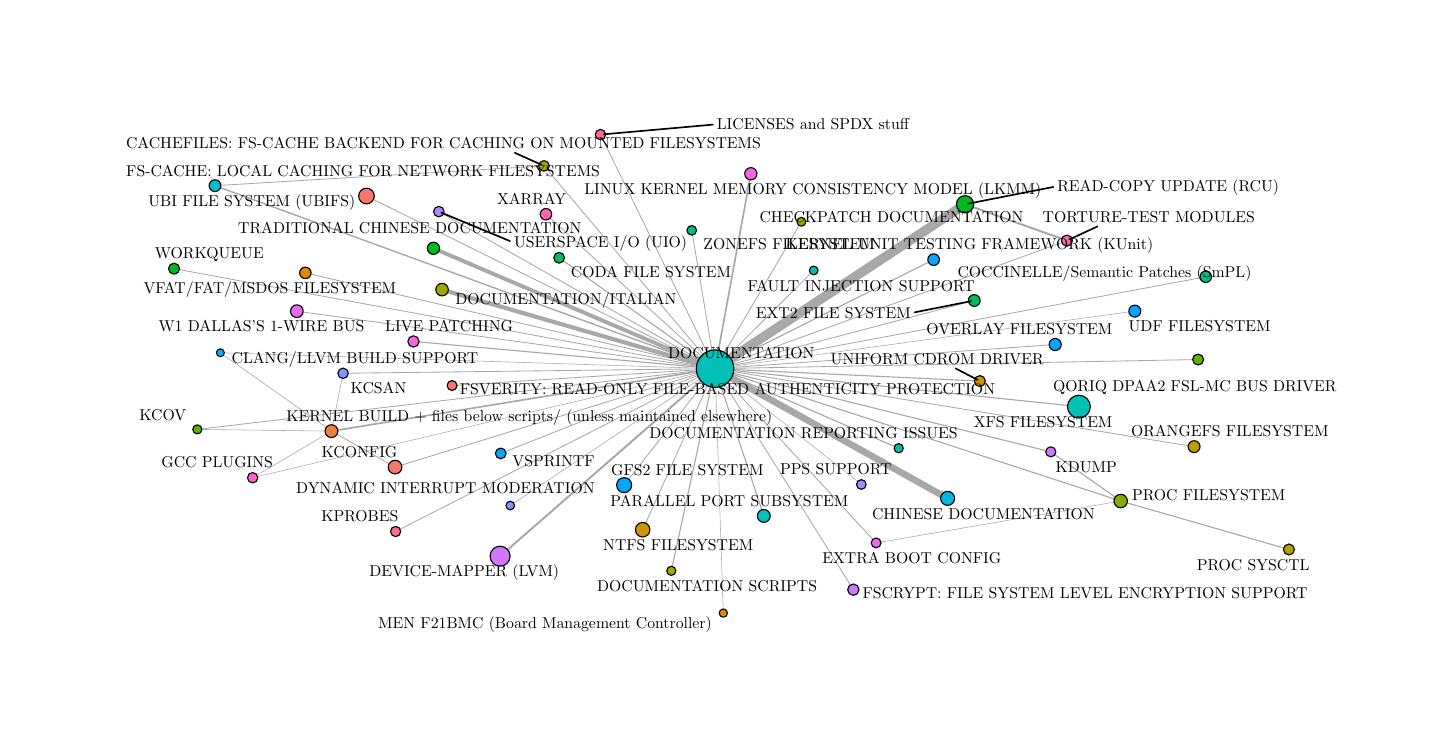
\begin{tikzpicture}[x=1pt,y=1pt]
\definecolor{fillColor}{RGB}{255,255,255}
\path[use as bounding box,fill=fillColor,fill opacity=0.00] (0,0) rectangle (505.89,252.94);
\begin{scope}
\path[clip] (  0.00,  0.00) rectangle (505.89,252.94);
\definecolor{fillColor}{RGB}{255,255,255}

\path[fill=fillColor] (  0.00,  0.00) rectangle (505.89,252.94);
\end{scope}
\begin{scope}
\path[clip] ( 32.75, 32.75) rectangle (475.89,222.94);
\definecolor{drawColor}{gray}{0.66}

\path[draw=drawColor,line width= 0.3pt,line join=round] (186.57,202.99) -- (248.39,129.72);

\path[draw=drawColor,line width= 0.3pt,line join=round] (186.57,202.99) -- ( 67.69,195.84);

\path[draw=drawColor,line width= 0.3pt,line join=round] (279.57,182.80) -- (248.39,129.72);

\path[draw=drawColor,line width= 2.4pt,line join=round] (332.42, 82.85) -- (248.39,129.72);

\path[draw=drawColor,line width= 0.2pt,line join=round] ( 69.63,135.47) -- (248.39,129.72);

\path[draw=drawColor,line width= 0.2pt,line join=round] ( 69.63,135.47) -- (109.77,107.15);

\path[draw=drawColor,line width= 0.3pt,line join=round] (425.70,162.92) -- (248.39,129.72);

\path[draw=drawColor,line width= 0.4pt,line join=round] (192.04,169.79) -- (248.39,129.72);

\path[draw=drawColor,line width= 0.7pt,line join=round] (170.71, 61.95) -- (248.39,129.72);

\path[draw=drawColor,line width= 0.4pt,line join=round] (248.39,129.72) -- (314.73,100.97);

\path[draw=drawColor,line width= 0.4pt,line join=round] (248.39,129.72) -- (232.58, 56.67);

\path[draw=drawColor,line width= 1.5pt,line join=round] (248.39,129.72) -- (149.73,158.29);

\path[draw=drawColor,line width= 0.2pt,line join=round] (248.39,129.72) -- (174.38, 80.26);

\path[draw=drawColor,line width= 0.3pt,line join=round] (248.39,129.72) -- (342.05,154.35);

\path[draw=drawColor,line width= 0.3pt,line join=round] (248.39,129.72) -- (306.58, 66.76);

\path[draw=drawColor,line width= 0.3pt,line join=round] (248.39,129.72) -- (284.03,165.21);

\path[draw=drawColor,line width= 0.5pt,line join=round] (248.39,129.72) -- ( 67.69,195.84);

\path[draw=drawColor,line width= 0.3pt,line join=round] (248.39,129.72) -- (298.35, 49.87);

\path[draw=drawColor,line width= 0.3pt,line join=round] (248.39,129.72) -- (153.35,123.63);

\path[draw=drawColor,line width= 0.2pt,line join=round] (248.39,129.72) -- ( 81.29, 90.31);

\path[draw=drawColor,line width= 0.3pt,line join=round] (248.39,129.72) -- (215.54, 87.64);

\path[draw=drawColor,line width= 0.3pt,line join=round] (248.39,129.72) -- (132.76, 94.15);

\path[draw=drawColor,line width= 0.3pt,line join=round] (248.39,129.72) -- ( 61.30,107.78);

\path[draw=drawColor,line width= 0.3pt,line join=round] (248.39,129.72) -- (113.97,128.05);

\path[draw=drawColor,line width= 0.4pt,line join=round] (248.39,129.72) -- (369.71, 99.67);

\path[draw=drawColor,line width= 0.6pt,line join=round] (248.39,129.72) -- (109.77,107.15);

\path[draw=drawColor,line width= 0.4pt,line join=round] (248.39,129.72) -- (327.36,169.12);

\path[draw=drawColor,line width= 0.3pt,line join=round] (248.39,129.72) -- (132.96, 70.88);

\path[draw=drawColor,line width= 0.3pt,line join=round] (248.39,129.72) -- (206.98,214.30);

\path[draw=drawColor,line width= 0.6pt,line join=round] (248.39,129.72) -- (261.32,200.15);

\path[draw=drawColor,line width= 0.4pt,line join=round] (248.39,129.72) -- (139.41,139.56);

\path[draw=drawColor,line width= 0.2pt,line join=round] (248.39,129.72) -- (251.37, 41.40);

\path[draw=drawColor,line width= 0.3pt,line join=round] (248.39,129.72) -- (222.23, 71.52);

\path[draw=drawColor,line width= 0.3pt,line join=round] (248.39,129.72) -- (421.48,101.54);

\path[draw=drawColor,line width= 0.3pt,line join=round] (248.39,129.72) -- (371.30,138.45);

\path[draw=drawColor,line width= 0.4pt,line join=round] (248.39,129.72) -- (265.99, 76.52);

\path[draw=drawColor,line width= 0.2pt,line join=round] (248.39,129.72) -- (301.24, 87.87);

\path[draw=drawColor,line width= 0.4pt,line join=round] (248.39,129.72) -- (394.96, 81.89);

\path[draw=drawColor,line width= 0.3pt,line join=round] (248.39,129.72) -- (422.93,133.02);

\path[draw=drawColor,line width= 3.4pt,line join=round] (248.39,129.72) -- (338.72,189.12);

\path[draw=drawColor,line width= 0.3pt,line join=round] (248.39,129.72) -- (375.53,176.00);

\path[draw=drawColor,line width= 1.4pt,line join=round] (248.39,129.72) -- (146.62,173.22);

\path[draw=drawColor,line width= 0.3pt,line join=round] (248.39,129.72) -- (122.42,192.10);

\path[draw=drawColor,line width= 0.2pt,line join=round] (248.39,129.72) -- (400.05,150.52);

\path[draw=drawColor,line width= 0.4pt,line join=round] (248.39,129.72) -- (344.07,125.24);

\path[draw=drawColor,line width= 0.3pt,line join=round] (248.39,129.72) -- (148.57,186.47);

\path[draw=drawColor,line width= 0.3pt,line join=round] (248.39,129.72) -- (100.34,164.34);

\path[draw=drawColor,line width= 0.3pt,line join=round] (248.39,129.72) -- (170.93, 99.10);

\path[draw=drawColor,line width= 0.3pt,line join=round] (248.39,129.72) -- ( 97.26,150.49);

\path[draw=drawColor,line width= 0.3pt,line join=round] (248.39,129.72) -- ( 52.89,165.86);

\path[draw=drawColor,line width= 0.3pt,line join=round] (248.39,129.72) -- (187.28,185.52);

\path[draw=drawColor,line width= 0.4pt,line join=round] (248.39,129.72) -- (379.86,116.00);

\path[draw=drawColor,line width= 0.3pt,line join=round] (248.39,129.72) -- (239.96,179.70);

\path[draw=drawColor,line width= 0.2pt,line join=round] (306.58, 66.76) -- (394.96, 81.89);

\path[draw=drawColor,line width= 0.2pt,line join=round] ( 81.29, 90.31) -- (109.77,107.15);

\path[draw=drawColor,line width= 0.3pt,line join=round] (132.76, 94.15) -- (109.77,107.15);

\path[draw=drawColor,line width= 0.2pt,line join=round] ( 61.30,107.78) -- (109.77,107.15);

\path[draw=drawColor,line width= 0.2pt,line join=round] (113.97,128.05) -- (109.77,107.15);

\path[draw=drawColor,line width= 0.4pt,line join=round] (369.71, 99.67) -- (394.96, 81.89);

\path[draw=drawColor,line width= 0.4pt,line join=round] (394.96, 81.89) -- (455.75, 64.38);

\path[draw=drawColor,line width= 0.7pt,line join=round] (338.72,189.12) -- (375.53,176.00);
\definecolor{drawColor}{RGB}{0,0,0}
\definecolor{fillColor}{RGB}{163,165,0}

\path[draw=drawColor,line width= 0.4pt,line join=round,line cap=round,fill=fillColor] (186.57,202.99) circle (  1.93);

\path[draw=drawColor,line width= 0.4pt,line join=round,line cap=round,fill=fillColor] (279.57,182.80) circle (  1.60);
\definecolor{fillColor}{RGB}{0,184,229}

\path[draw=drawColor,line width= 0.4pt,line join=round,line cap=round,fill=fillColor] (332.42, 82.85) circle (  2.53);
\definecolor{fillColor}{RGB}{0,176,246}

\path[draw=drawColor,line width= 0.4pt,line join=round,line cap=round,fill=fillColor] ( 69.63,135.47) circle (  1.43);
\definecolor{fillColor}{RGB}{0,191,125}

\path[draw=drawColor,line width= 0.4pt,line join=round,line cap=round,fill=fillColor] (425.70,162.92) circle (  2.07);
\definecolor{fillColor}{RGB}{0,188,89}

\path[draw=drawColor,line width= 0.4pt,line join=round,line cap=round,fill=fillColor] (192.04,169.79) circle (  1.95);
\definecolor{fillColor}{RGB}{207,120,255}

\path[draw=drawColor,line width= 0.4pt,line join=round,line cap=round,fill=fillColor] (170.71, 61.95) circle (  3.61);
\definecolor{fillColor}{RGB}{0,192,184}

\path[draw=drawColor,line width= 0.4pt,line join=round,line cap=round,fill=fillColor] (248.39,129.72) circle (  6.78);
\definecolor{fillColor}{RGB}{0,193,156}

\path[draw=drawColor,line width= 0.4pt,line join=round,line cap=round,fill=fillColor] (314.73,100.97) circle (  1.67);
\definecolor{fillColor}{RGB}{163,165,0}

\path[draw=drawColor,line width= 0.4pt,line join=round,line cap=round,fill=fillColor] (232.58, 56.67) circle (  1.66);

\path[draw=drawColor,line width= 0.4pt,line join=round,line cap=round,fill=fillColor] (149.73,158.29) circle (  2.26);
\definecolor{fillColor}{RGB}{121,151,255}

\path[draw=drawColor,line width= 0.4pt,line join=round,line cap=round,fill=fillColor] (174.38, 80.26) circle (  1.56);
\definecolor{fillColor}{RGB}{0,188,89}

\path[draw=drawColor,line width= 0.4pt,line join=round,line cap=round,fill=fillColor] (342.05,154.35) circle (  2.12);
\definecolor{fillColor}{RGB}{231,107,243}

\path[draw=drawColor,line width= 0.4pt,line join=round,line cap=round,fill=fillColor] (306.58, 66.76) circle (  1.78);
\definecolor{fillColor}{RGB}{0,192,184}

\path[draw=drawColor,line width= 0.4pt,line join=round,line cap=round,fill=fillColor] (284.03,165.21) circle (  1.58);
\definecolor{fillColor}{RGB}{0,189,208}

\path[draw=drawColor,line width= 0.4pt,line join=round,line cap=round,fill=fillColor] ( 67.69,195.84) circle (  2.13);
\definecolor{fillColor}{RGB}{207,120,255}

\path[draw=drawColor,line width= 0.4pt,line join=round,line cap=round,fill=fillColor] (298.35, 49.87) circle (  2.05);
\definecolor{fillColor}{RGB}{248,118,109}

\path[draw=drawColor,line width= 0.4pt,line join=round,line cap=round,fill=fillColor] (153.35,123.63) circle (  1.80);
\definecolor{fillColor}{RGB}{255,97,201}

\path[draw=drawColor,line width= 0.4pt,line join=round,line cap=round,fill=fillColor] ( 81.29, 90.31) circle (  1.87);
\definecolor{fillColor}{RGB}{0,165,255}

\path[draw=drawColor,line width= 0.4pt,line join=round,line cap=round,fill=fillColor] (215.54, 87.64) circle (  2.71);
\definecolor{fillColor}{RGB}{248,118,109}

\path[draw=drawColor,line width= 0.4pt,line join=round,line cap=round,fill=fillColor] (132.76, 94.15) circle (  2.47);
\definecolor{fillColor}{RGB}{91,179,0}

\path[draw=drawColor,line width= 0.4pt,line join=round,line cap=round,fill=fillColor] ( 61.30,107.78) circle (  1.65);
\definecolor{fillColor}{RGB}{121,151,255}

\path[draw=drawColor,line width= 0.4pt,line join=round,line cap=round,fill=fillColor] (113.97,128.05) circle (  1.89);
\definecolor{fillColor}{RGB}{207,120,255}

\path[draw=drawColor,line width= 0.4pt,line join=round,line cap=round,fill=fillColor] (369.71, 99.67) circle (  1.83);
\definecolor{fillColor}{RGB}{237,129,65}

\path[draw=drawColor,line width= 0.4pt,line join=round,line cap=round,fill=fillColor] (109.77,107.15) circle (  2.31);
\definecolor{fillColor}{RGB}{0,165,255}

\path[draw=drawColor,line width= 0.4pt,line join=round,line cap=round,fill=fillColor] (327.36,169.12) circle (  2.10);
\definecolor{fillColor}{RGB}{255,108,144}

\path[draw=drawColor,line width= 0.4pt,line join=round,line cap=round,fill=fillColor] (132.96, 70.88) circle (  1.85);

\path[draw=drawColor,line width= 0.4pt,line join=round,line cap=round,fill=fillColor] (206.98,214.30) circle (  1.89);
\definecolor{fillColor}{RGB}{247,99,224}

\path[draw=drawColor,line width= 0.4pt,line join=round,line cap=round,fill=fillColor] (261.32,200.15) circle (  2.21);

\path[draw=drawColor,line width= 0.4pt,line join=round,line cap=round,fill=fillColor] (139.41,139.56) circle (  2.05);
\definecolor{fillColor}{RGB}{224,139,0}

\path[draw=drawColor,line width= 0.4pt,line join=round,line cap=round,fill=fillColor] (251.37, 41.40) circle (  1.50);
\definecolor{fillColor}{RGB}{207,148,0}

\path[draw=drawColor,line width= 0.4pt,line join=round,line cap=round,fill=fillColor] (222.23, 71.52) circle (  2.62);
\definecolor{fillColor}{RGB}{187,157,0}

\path[draw=drawColor,line width= 0.4pt,line join=round,line cap=round,fill=fillColor] (421.48,101.54) circle (  2.15);
\definecolor{fillColor}{RGB}{0,165,255}

\path[draw=drawColor,line width= 0.4pt,line join=round,line cap=round,fill=fillColor] (371.30,138.45) circle (  2.19);
\definecolor{fillColor}{RGB}{0,192,184}

\path[draw=drawColor,line width= 0.4pt,line join=round,line cap=round,fill=fillColor] (265.99, 76.52) circle (  2.33);
\definecolor{fillColor}{RGB}{172,136,255}

\path[draw=drawColor,line width= 0.4pt,line join=round,line cap=round,fill=fillColor] (301.24, 87.87) circle (  1.75);
\definecolor{fillColor}{RGB}{133,173,0}

\path[draw=drawColor,line width= 0.4pt,line join=round,line cap=round,fill=fillColor] (394.96, 81.89) circle (  2.43);
\definecolor{fillColor}{RGB}{187,157,0}

\path[draw=drawColor,line width= 0.4pt,line join=round,line cap=round,fill=fillColor] (455.75, 64.38) circle (  1.99);
\definecolor{fillColor}{RGB}{91,179,0}

\path[draw=drawColor,line width= 0.4pt,line join=round,line cap=round,fill=fillColor] (422.93,133.02) circle (  1.99);
\definecolor{fillColor}{RGB}{0,184,31}

\path[draw=drawColor,line width= 0.4pt,line join=round,line cap=round,fill=fillColor] (338.72,189.12) circle (  3.12);
\definecolor{fillColor}{RGB}{255,101,174}

\path[draw=drawColor,line width= 0.4pt,line join=round,line cap=round,fill=fillColor] (375.53,176.00) circle (  2.01);
\definecolor{fillColor}{RGB}{0,184,31}

\path[draw=drawColor,line width= 0.4pt,line join=round,line cap=round,fill=fillColor] (146.62,173.22) circle (  2.21);
\definecolor{fillColor}{RGB}{248,118,109}

\path[draw=drawColor,line width= 0.4pt,line join=round,line cap=round,fill=fillColor] (122.42,192.10) circle (  2.83);
\definecolor{fillColor}{RGB}{0,165,255}

\path[draw=drawColor,line width= 0.4pt,line join=round,line cap=round,fill=fillColor] (400.05,150.52) circle (  2.16);
\definecolor{fillColor}{RGB}{207,148,0}

\path[draw=drawColor,line width= 0.4pt,line join=round,line cap=round,fill=fillColor] (344.07,125.24) circle (  1.98);
\definecolor{fillColor}{RGB}{172,136,255}

\path[draw=drawColor,line width= 0.4pt,line join=round,line cap=round,fill=fillColor] (148.57,186.47) circle (  1.90);
\definecolor{fillColor}{RGB}{224,139,0}

\path[draw=drawColor,line width= 0.4pt,line join=round,line cap=round,fill=fillColor] (100.34,164.34) circle (  2.07);
\definecolor{fillColor}{RGB}{0,165,255}

\path[draw=drawColor,line width= 0.4pt,line join=round,line cap=round,fill=fillColor] (170.93, 99.10) circle (  1.94);
\definecolor{fillColor}{RGB}{231,107,243}

\path[draw=drawColor,line width= 0.4pt,line join=round,line cap=round,fill=fillColor] ( 97.26,150.49) circle (  2.29);
\definecolor{fillColor}{RGB}{0,184,31}

\path[draw=drawColor,line width= 0.4pt,line join=round,line cap=round,fill=fillColor] ( 52.89,165.86) circle (  2.00);
\definecolor{fillColor}{RGB}{255,101,174}

\path[draw=drawColor,line width= 0.4pt,line join=round,line cap=round,fill=fillColor] (187.28,185.52) circle (  2.07);
\definecolor{fillColor}{RGB}{0,192,184}

\path[draw=drawColor,line width= 0.4pt,line join=round,line cap=round,fill=fillColor] (379.86,116.00) circle (  4.13);
\definecolor{fillColor}{RGB}{0,191,125}

\path[draw=drawColor,line width= 0.4pt,line join=round,line cap=round,fill=fillColor] (239.96,179.70) circle (  1.74);

\path[draw=drawColor,line width= 0.6pt,line join=round,line cap=round] (176.05,207.71) -- (185.69,203.38);

\path[draw=drawColor,line width= 0.6pt,line join=round,line cap=round] (320.58,150.09) -- (340.90,154.12);

\path[draw=drawColor,line width= 0.6pt,line join=round,line cap=round] (247.58,217.90) -- (208.22,214.41);

\path[draw=drawColor,line width= 0.6pt,line join=round,line cap=round] (370.65,195.39) -- (339.88,189.35);

\path[draw=drawColor,line width= 0.6pt,line join=round,line cap=round] (386.58,181.12) -- (376.39,176.40);

\path[draw=drawColor,line width= 0.6pt,line join=round,line cap=round] (335.28,129.83) -- (343.26,125.66);

\path[draw=drawColor,line width= 0.6pt,line join=round,line cap=round] (174.30,175.82) -- (149.49,186.09);

\node[text=drawColor,anchor=base,inner sep=0pt, outer sep=0pt, scale=  0.57] at (150.25,209.21) {CACHEFILES: FS-CACHE BACKEND FOR CACHING ON MOUNTED FILESYSTEMS};

\node[text=drawColor,anchor=base,inner sep=0pt, outer sep=0pt, scale=  0.57] at (312.14,182.68) {CHECKPATCH DOCUMENTATION};

\node[text=drawColor,anchor=base,inner sep=0pt, outer sep=0pt, scale=  0.57] at (345.35, 75.35) {CHINESE DOCUMENTATION};

\node[text=drawColor,anchor=base,inner sep=0pt, outer sep=0pt, scale=  0.57] at (118.26,131.64) {CLANG/LLVM BUILD SUPPORT};

\node[text=drawColor,anchor=base,inner sep=0pt, outer sep=0pt, scale=  0.57] at (389.10,162.74) {COCCINELLE/Semantic Patches (SmPL)};

\node[text=drawColor,anchor=base,inner sep=0pt, outer sep=0pt, scale=  0.57] at (225.25,162.84) {CODA FILE SYSTEM};

\node[text=drawColor,anchor=base,inner sep=0pt, outer sep=0pt, scale=  0.57] at (157.76, 54.46) {DEVICE-MAPPER  (LVM)};

\node[text=drawColor,anchor=base,inner sep=0pt, outer sep=0pt, scale=  0.57] at (257.84,133.30) {DOCUMENTATION};

\node[text=drawColor,anchor=base,inner sep=0pt, outer sep=0pt, scale=  0.57] at (280.34,104.53) {DOCUMENTATION REPORTING ISSUES};

\node[text=drawColor,anchor=base,inner sep=0pt, outer sep=0pt, scale=  0.57] at (245.50, 49.17) {DOCUMENTATION SCRIPTS};

\node[text=drawColor,anchor=base,inner sep=0pt, outer sep=0pt, scale=  0.57] at (194.51,152.91) {DOCUMENTATION/ITALIAN};

\node[text=drawColor,anchor=base,inner sep=0pt, outer sep=0pt, scale=  0.57] at (150.96, 84.45) {DYNAMIC INTERRUPT MODERATION};

\node[text=drawColor,anchor=base,inner sep=0pt, outer sep=0pt, scale=  0.57] at (291.14,147.78) {EXT2 FILE SYSTEM};

\node[text=drawColor,anchor=base,inner sep=0pt, outer sep=0pt, scale=  0.57] at (319.47, 59.28) {EXTRA BOOT CONFIG};

\node[text=drawColor,anchor=base,inner sep=0pt, outer sep=0pt, scale=  0.57] at (301.19,157.73) {FAULT INJECTION SUPPORT};

\node[text=drawColor,anchor=base,inner sep=0pt, outer sep=0pt, scale=  0.57] at (121.21,199.22) {FS-CACHE: LOCAL CACHING FOR NETWORK FILESYSTEMS};

\node[text=drawColor,anchor=base,inner sep=0pt, outer sep=0pt, scale=  0.57] at (382.06, 46.82) {FSCRYPT: FILE SYSTEM LEVEL ENCRYPTION SUPPORT};

\node[text=drawColor,anchor=base,inner sep=0pt, outer sep=0pt, scale=  0.57] at (252.88,120.56) {FSVERITY: READ-ONLY FILE-BASED AUTHENTICITY PROTECTION};

\node[text=drawColor,anchor=base,inner sep=0pt, outer sep=0pt, scale=  0.57] at ( 68.48, 93.87) {GCC PLUGINS};

\node[text=drawColor,anchor=base,inner sep=0pt, outer sep=0pt, scale=  0.57] at (238.37, 91.20) {GFS2 FILE SYSTEM};

\node[text=drawColor,anchor=base,inner sep=0pt, outer sep=0pt, scale=  0.57] at (119.91, 97.72) {KCONFIG};

\node[text=drawColor,anchor=base,inner sep=0pt, outer sep=0pt, scale=  0.57] at ( 48.85,111.16) {KCOV};

\node[text=drawColor,anchor=base,inner sep=0pt, outer sep=0pt, scale=  0.57] at (126.78,120.60) {KCSAN};

\node[text=drawColor,anchor=base,inner sep=0pt, outer sep=0pt, scale=  0.57] at (382.52, 92.22) {KDUMP};

\node[text=drawColor,anchor=base,inner sep=0pt, outer sep=0pt, scale=  0.57] at (181.23,110.62) {KERNEL BUILD + files below scripts/ (unless maintained elsewhere)};

\node[text=drawColor,anchor=base,inner sep=0pt, outer sep=0pt, scale=  0.57] at (340.29,172.71) {KERNEL UNIT TESTING FRAMEWORK (KUnit)};

\node[text=drawColor,anchor=base,inner sep=0pt, outer sep=0pt, scale=  0.57] at (120.03, 74.45) {KPROBES};

\node[text=drawColor,anchor=base,inner sep=0pt, outer sep=0pt, scale=  0.57] at (283.76,216.01) {LICENSES and SPDX stuff};

\node[text=drawColor,anchor=base,inner sep=0pt, outer sep=0pt, scale=  0.57] at (283.72,192.67) {LINUX KERNEL MEMORY CONSISTENCY MODEL (LKMM)};

\node[text=drawColor,anchor=base,inner sep=0pt, outer sep=0pt, scale=  0.57] at (152.29,143.13) {LIVE PATCHING};

\node[text=drawColor,anchor=base,inner sep=0pt, outer sep=0pt, scale=  0.57] at (186.93, 35.76) {MEN F21BMC (Board Management Controller)};

\node[text=drawColor,anchor=base,inner sep=0pt, outer sep=0pt, scale=  0.57] at (235.09, 64.02) {NTFS FILESYSTEM};

\node[text=drawColor,anchor=base,inner sep=0pt, outer sep=0pt, scale=  0.57] at (434.38,105.09) {ORANGEFS FILESYSTEM};

\node[text=drawColor,anchor=base,inner sep=0pt, outer sep=0pt, scale=  0.57] at (358.37,142.01) {OVERLAY FILESYSTEM};

\node[text=drawColor,anchor=base,inner sep=0pt, outer sep=0pt, scale=  0.57] at (253.56, 80.09) {PARALLEL PORT SUBSYSTEM};

\node[text=drawColor,anchor=base,inner sep=0pt, outer sep=0pt, scale=  0.57] at (292.01, 91.44) {PPS SUPPORT};

\node[text=drawColor,anchor=base,inner sep=0pt, outer sep=0pt, scale=  0.57] at (426.77, 82.21) {PROC FILESYSTEM};

\node[text=drawColor,anchor=base,inner sep=0pt, outer sep=0pt, scale=  0.57] at (442.84, 56.87) {PROC SYSCTL};

\node[text=drawColor,anchor=base,inner sep=0pt, outer sep=0pt, scale=  0.57] at (421.75,121.41) {QORIQ DPAA2 FSL-MC BUS DRIVER};

\node[text=drawColor,anchor=base,inner sep=0pt, outer sep=0pt, scale=  0.57] at (412.14,193.69) {READ-COPY UPDATE (RCU)};

\node[text=drawColor,anchor=base,inner sep=0pt, outer sep=0pt, scale=  0.57] at (405.13,182.62) {TORTURE-TEST MODULES};

\node[text=drawColor,anchor=base,inner sep=0pt, outer sep=0pt, scale=  0.57] at (138.11,178.41) {TRADITIONAL CHINESE DOCUMENTATION};

\node[text=drawColor,anchor=base,inner sep=0pt, outer sep=0pt, scale=  0.57] at ( 81.01,188.36) {UBI FILE SYSTEM (UBIFS)};

\node[text=drawColor,anchor=base,inner sep=0pt, outer sep=0pt, scale=  0.57] at (423.48,143.05) {UDF FILESYSTEM};

\node[text=drawColor,anchor=base,inner sep=0pt, outer sep=0pt, scale=  0.57] at (328.65,131.34) {UNIFORM CDROM DRIVER};

\node[text=drawColor,anchor=base,inner sep=0pt, outer sep=0pt, scale=  0.57] at (207.02,173.37) {USERSPACE I/O (UIO)};

\node[text=drawColor,anchor=base,inner sep=0pt, outer sep=0pt, scale=  0.57] at ( 87.53,156.86) {VFAT/FAT/MSDOS FILESYSTEM};

\node[text=drawColor,anchor=base,inner sep=0pt, outer sep=0pt, scale=  0.57] at (190.01, 94.39) {VSPRINTF};

\node[text=drawColor,anchor=base,inner sep=0pt, outer sep=0pt, scale=  0.57] at ( 84.49,143.04) {W1 DALLAS'S 1-WIRE BUS};

\node[text=drawColor,anchor=base,inner sep=0pt, outer sep=0pt, scale=  0.57] at ( 65.65,169.42) {WORKQUEUE};

\node[text=drawColor,anchor=base,inner sep=0pt, outer sep=0pt, scale=  0.57] at (182.10,189.06) {XARRAY};

\node[text=drawColor,anchor=base,inner sep=0pt, outer sep=0pt, scale=  0.57] at (366.93,108.48) {XFS FILESYSTEM};

\node[text=drawColor,anchor=base,inner sep=0pt, outer sep=0pt, scale=  0.57] at (275.15,172.72) {ZONEFS FILESYSTEM};
\end{scope}
\end{tikzpicture}
